\documentclass{beamer}

\usepackage[T1]{fontenc}
\usepackage[utf8]{inputenc}
\usepackage[frenchb]{babel}
\usepackage{eurosym}

\usepackage{graphicx}


\newcommand\host{{\it host}\,}
\newcommand\device{{\it device}\,}


% --------- BEGIN STYLE BEAMER ---------
\usetheme{Madrid}
\definecolor{ECNBleu}{HTML}{102648}
\definecolor{ECNJaune}{HTML}{FAB600}

\setbeamercolor{frametitle}{bg=ECNBleu,fg=white} %le titre de la frame, en haut
\setbeamercolor{title in head/foot}{bg=ECNJaune,fg=ECNBleu} %barre bas, milieu
\setbeamercolor{author in head/foot}{bg=ECNBleu,fg=ECNJaune} %barre bas, gauche
\setbeamercolor{date in head/foot}{bg=ECNBleu,fg=ECNJaune} %barre bas, droit
\setbeamercolor{section in head/foot}{bg=ECNJaune,fg=ECNBleu} %haut gauche
\setbeamercolor{subsection in head/foot}{bg=ECNBleu,fg=ECNBleu} %haut droite
\setbeamercolor{title}{bg=ECNBleu,fg=white}
\setbeamercolor{block title}{fg=white,bg=ECNBleu}

%\setbeamercolor{normal text}{bg=IUTBleuFonce} %texte
\setbeamercolor{item}{bg=ECNBleu}
\setbeamercolor{subitem}{bg=ECNJaune}
\setbeamercolor{description item}{fg=couleurEmph}
\setbeamercolor{section in toc}{fg=ECNBleu}
%\setbeamercolor{subsubitem}{bg=IUTBleuFonce}

%structure (eq emph dans beamer)
\setbeamercolor{emph}{fg=couleurEmph}
% ----------------------------

\usepackage{listings}

\lstdefinestyle{customc}{
  belowcaptionskip=1\baselineskip,
  breaklines=true,
  frame=L,
  xleftmargin=\parindent,
  language=C,
  showstringspaces=false,
  basicstyle=\tiny\ttfamily,
  keywordstyle=\bfseries\color{green!40!black},
  commentstyle=\itshape\color{purple!40!black},
  identifierstyle=\color{blue},
  stringstyle=\color{orange},
}

\lstset{escapechar=@,style=customc}

\newenvironment<>{questionblock}[1]{%
\setbeamercolor{block title}{bg=ECNJaune,fg=ECNBleu}%
\begin{block}#2{#1}}{\end{block}}

\title[GPGPU]{Programmation sur Processeur Graphique}
\subtitle[\ldots]{---\\Part 1 : Introduction à la programmation parallèle}
\author[P.-E. Hladik]{Pierre-Emmanuel Hladik\\\tiny pierre-emmanuel.hladik@ec-nantes.fr}
\institute[Centrale Nantes]{}
%{\tiny\date{\today}}
%\logo{
\titlegraphic{
	\flushleft
\includegraphics[width=3cm]{./LogoCN_RVB}
}

\begin{document}

 \frame{\titlepage}
 

%%%%%%%%%%%%%%%%%%%%%%%%%%%
\section{Introduction à la programmation parallèle}
\subsection{Architecture parallèle}
\begin{frame}{Plan}
\tableofcontents[sections={1-4}, currentsubsection]
\end{frame}
%%%%%%%%%%%%%%%%%%%%%%%%%%%


%%%%%%%%%%%%%%%%%%%%%%%%%%
\begin{frame}[plain]
\frametitle{Exemple d'architecture hétérogène parallèle}
	\begin{center}
	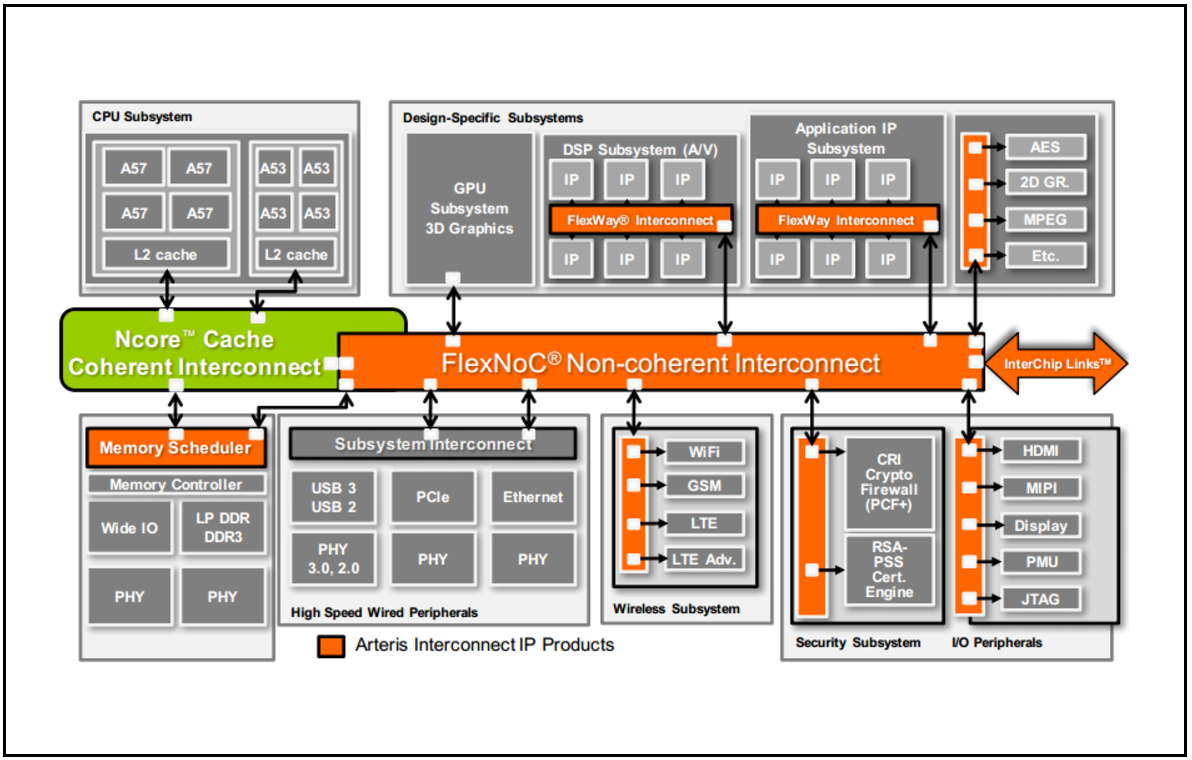
\includegraphics[scale=0.5]{./figures-pdf/heterogeneous}<1>
	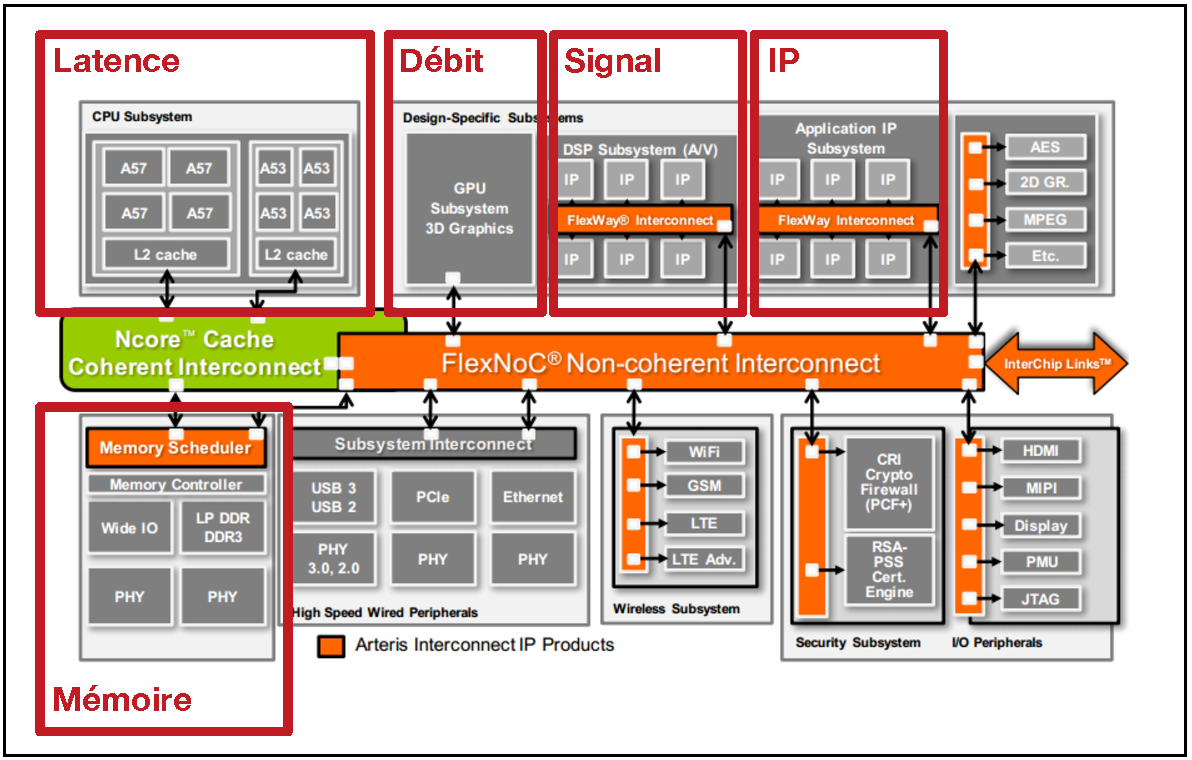
\includegraphics[scale=0.5]{./figures-pdf/heterogeneous2}<2>
	
	{\tiny \url{https://www.arteris.com/hubfs/2016-05-24-arteris-ncore-overview-PDF-FINAL.pdf}}
	\end{center}
\end{frame}



%%%%%%%%%%%%%%%%%%%%%%%%%%
\begin{frame}[plain]
\frametitle{Architecture CPU}

    \begin{block}{CPU : Latency Oriented Design (latence)}
    Optimisé pour les performances d'un {\bf code séquentiel}.
	\begin{center}
	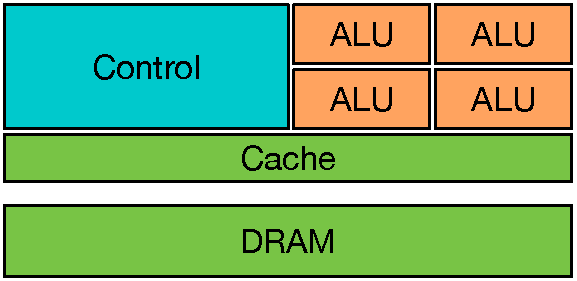
\includegraphics[scale=0.4]{./figures-pdf/cpu}
	\end{center}

\begin{itemize}
\item ALU puissante : réduction de la latence des opérations
\item Larges caches : conversion des accès longs à la mémoire en des accès courts au cache (réduction de la latence)
\item Contrôle d'exécution sophistiqués : prédiction de branchement, pipeline, data forwarding, etc. pour réduire la latence 
\end{itemize}
   	  \end{block}   
\end{frame}

%%%%%%%%%%%%%%%%%%%%%%%%%%
\begin{frame}[plain]
\frametitle{Architecture GPU}	  
    \begin{block}{GPU : Throughput Oriented Design (débit)}
    Optimisé pour les performances d'un {\bf code parallèle} (augmente le débit, c.-à-d. le travail réalisé par unité de temps).
	\begin{center}
	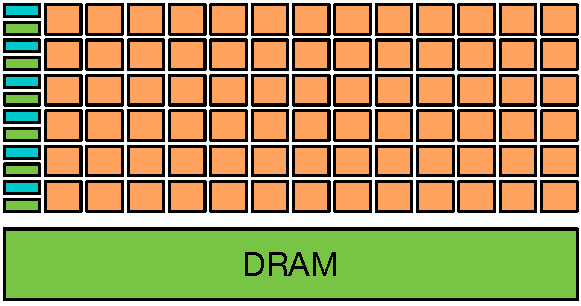
\includegraphics[scale=0.4]{./figures-pdf/gpu}
	\end{center}

\begin{itemize}
\item Petites caches : accélération du débit mémoire
\item Contrôle simple : pas de prédiction de branchement, pas de data forwarding 
\item ALU : nombreuses unités, latence importante mais de nombreux pipeline pour un grand débit
\item Grand nombre de threads matériels
\end{itemize}

	  \end{block}   
\end{frame}

%%%%%%%%%%%%%%%%%%%%%%%%%%
\begin{frame}[plain]
\frametitle{Architecture CPU vs GPU}	  
\begin{columns}[t]
  \begin{column}{0.45\textwidth}
    \begin{block}{CPU}
	\begin{itemize}
		\item  pour les parties séquentielles où la latence est importante
		\item peut être 10x plus rapide qu'un GPU pour du code séquentiel
	\end{itemize}
\end{block}   
  \end{column}
  
  \begin{column}{0.45\textwidth}
    \begin{block}{GPU}
    	\begin{itemize}
		\item  pour les parties parallèles avec un haut débit souhaité
		\item peut être 10x plus rapide qu'un CPU pour le code parallèle
	\end{itemize}
    \end{block}  
  \end{column}
 \end{columns}
 
     \begin{block}{The winner is...}
     De bonnes performances pour une application s'obtient en utilisant judicieusement des CPU et des GPU.
    \end{block} 
   
\end{frame}
%%%%%%%%%%%%%%%%%%%%%%%%%%
\begin{frame}[plain]
\frametitle{Mais c'est quoi un traitement parallèle ?}

    \begin{block}{Traitement massivement parallèle}
    	En informatique, le traitement massivement parallèle (en anglais, {\it massively parallel processing} ou {\it massively parallel computing}) est l'utilisation d'un grand nombre de processeurs (ou d'ordinateurs distincts) pour effectuer un ensemble de calculs coordonnés en parallèle (c'est-à-dire {\bf simultanément}). [\href{https://fr.wikipedia.org/wiki/Traitement_massivement_parallèle}{wikipedia}]
     \end{block}   
\end{frame}
%%%%%%%%%%%%%%%%%%%%%%%%%%
%%%%%%%%%%%%%%%%%%%%%%%%%%
\begin{frame}[plain]
\frametitle{Focus sur la notion de thread}
%
\begin{block}{Thread}
Un thread est {\bf une exécution d'un programme séquentiel}.

Un thread est composé : du code, de son point d'exécution, et des valeurs de ses variables et structures de données.

Des API de programmation sont offertes pour créer et manipuler les threads.
\end{block}

\begin{block}{Exécution séquentielle}
Une opération se fait que lorsque l'opération précédente est terminée, y compris lorsque les deux opérations sont indépendantes.
\end{block}

\begin{alertblock}{}
Un thread ne peut pas être parallélisé.

Il faut au moins deux threads pour réaliser une exécution parallèle.
\end{alertblock}

\end{frame}
%%%%%%%%%%%%%%%%%%%%%%%%%%
\begin{frame}[plain]
\frametitle{Digression : concurrent vs parallèle}
%

\begin{block}{Exécution concurrente}
Si plusieurs threads sont actifs en même temps et que le système d'exploitation attribue la ressource de calcul aux threads en basculant d'un thread à un autre, on parle d'exécution concurrente.
\end{block}

\center
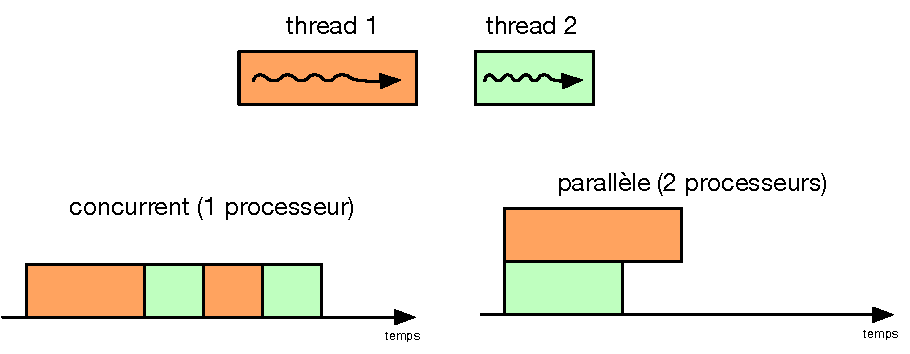
\includegraphics[scale=0.5]{./figures-pdf/concurrentVSparallele}

\begin{block}{Ordonnancement / ordonnanceur}
L'{\bf ordonnancement} est le fait d'ordonner les threads à exécuter.

Dans les systèmes d'exploitation, l'{\bf ordonnanceur} ({\it scheduler}) est le composant du noyau choisissant l'ordre d'exécution des threads.
\end{block}

\end{frame}
%%%%%%%%%%%%%%%%%%%%%%%%%%
\begin{frame}[plain]
\frametitle{Digression : un peu de cuisine}
%

\center
\includegraphics[scale=0.27]{./figures-pdf/cuisine}
\end{frame}

%%%%%%%%%%%%%%%%%%%%%%%%%%
\begin{frame}[plain]
\frametitle{Plusieurs type de parallélisme}
\begin{columns}[t]
  \begin{column}{0.45\textwidth}
    \begin{block}{Parallélisme de tâches}
    	\begin{itemize}
		\item décomposition de l'application en tâches
		\item les traitements des tâches sont indépendants
	\end{itemize}
     \end{block}   
  \end{column}
  
  \begin{column}{0.45\textwidth}
    \begin{block}{Parallélisme des données}
    	\begin{itemize}
		\item traitement des données en parallèle
		\item les traitements sont identiques
	\end{itemize}
	  \end{block}   
  \end{column}
 \end{columns}  
 
\end{frame}
%%%%%%%%%%%%%%%%%%%%%%%%%%
\begin{frame}[plain]
\frametitle{Taxonomie de Flynn (1966)}	  
	\begin{block}{}
La taxonomie de Flynn est une classification en quatre catégories des architectures d'ordinateur selon le type d'organisation du flux de données et du flux d'instructions.
	\end{block} 
	\bigskip
	\begin{center}
	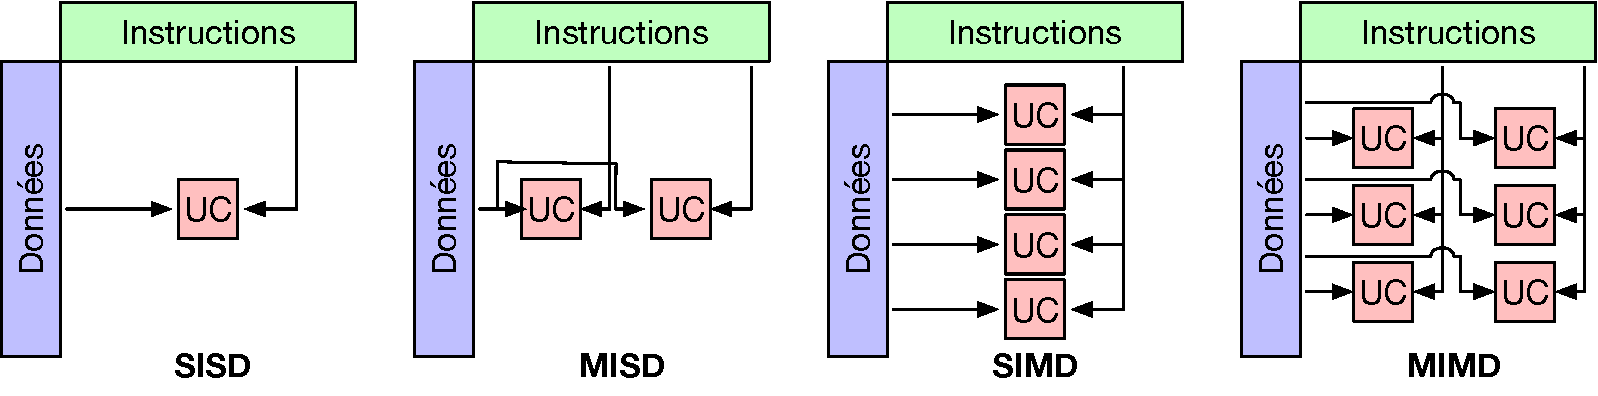
\includegraphics[scale=0.4]{./figures-pdf/flynn}
	\end{center}  

	\only<1>{
	\begin{block}{SISD (unique flux d'instructions, unique flux de données)}
	Ordinateur séquentiel qui n'exploite aucun parallélisme, tant au niveau des instructions qu'au niveau de la mémoire. Cette catégorie correspond à l'architecture de von Neumann.
	\end{block} 
	}

	\only<2>{
	\begin{block}{MISD (multiples flux d'instructions, unique flux de données)}
	Ordinateur dans lequel une même donnée est traitée par plusieurs unités de calcul en parallèle. Peu d'implémentations en pratique, utilisée dans le filtrage numérique et la vérification de redondance dans les systèmes critiques.
	\end{block} 
	}
	
	\only<3>{
	\begin{block}{SIMD (unique flux d'instructions, multiples flux de données)}
	Ordinateur qui utilise le parallélisme au niveau de la mémoire, par exemple le processeur vectoriel.
	\end{block} 
	}
	
	\only<4>{
	\begin{block}{MIMD (multiples flux d'instructions, multiples flux de données)}
	Plusieurs unités de calcul traitent des données différentes, car chacune d'elles possède une mémoire distincte. Il s'agit de l'architecture parallèle la plus utilisée pour les CPU modernes.
	\end{block} 
	}
	
\end{frame}


%%%%%%%%%%%%%%%%%%%%%%%%%%%
%\begin{frame}[plain]
%\frametitle{Exemple de traitement concurrent et parallèle}
%	\begin{center}
%	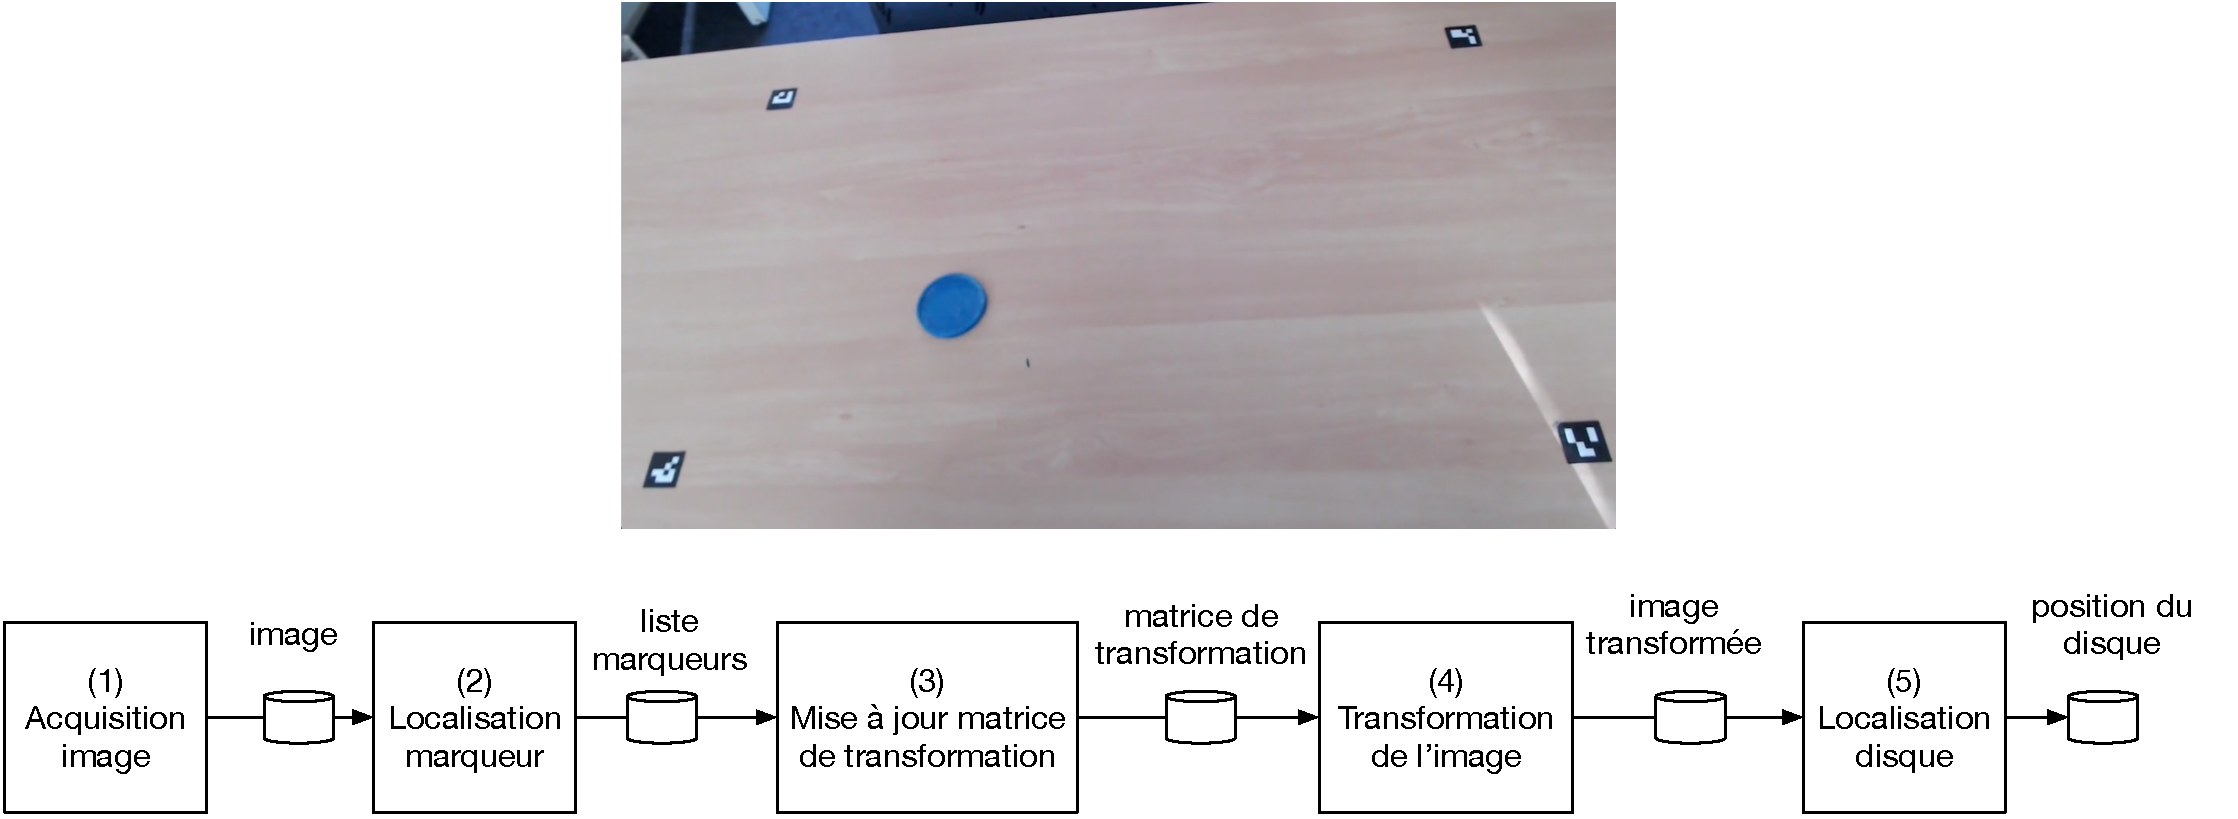
\includegraphics[width=\textwidth]{./figures-pdf/ahia}
%	\end{center}
%
%\end{frame}
%%%%%%%%%%%%%%%%%%%%%%%%%%%

%%%%%%%%%%%%%%%%%%%%%%%%%%%
\subsection{Remarque sur l'accélération}
\begin{frame}{Plan}
\tableofcontents[sections={1-4}, currentsubsection]
\end{frame}
%%%%%%%%%%%%%%%%%%%%%%%%%%%

%%%%%%%%%%%%%%%%%%%%%%%%%%
\begin{frame}[plain]
\frametitle{Loi d'Amdahl (1967)}
	\begin{center}
		$$S_{latence} = \frac{1}{1-p + \frac{p}{s}}$$
	\end{center}
	avec :
	\begin{itemize}
		\item $S_{latence}$ l'accélération ({\it speedup}) en latence de l'exécution
		\item $s$  le nombre de fils d'exécutions
		\item $p$  le pourcentage du temps d'exécution bénéficiant du parallèlisme
	\end{itemize}
	
  \uncover<2>{
		\begin{center}
		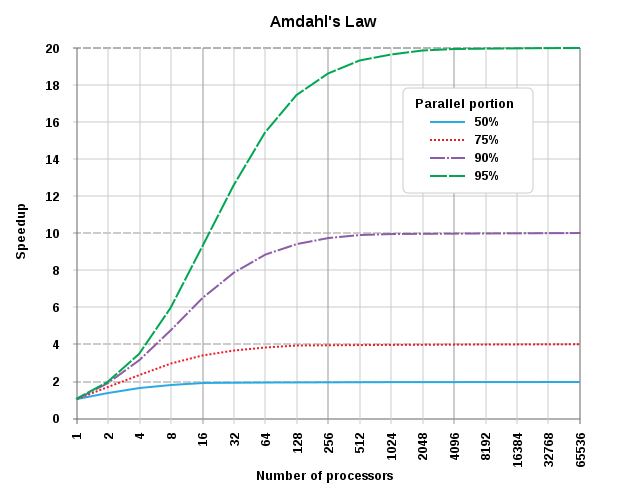
\includegraphics[scale=0.24]{./figures-pdf/AmdahlsLaw}
		{\tiny [\href{https://fr.wikipedia.org/wiki/Loi_d\%27Amdahl}{wikipedia}]}
	\end{center}
	}

\end{frame}
%%%%%%%%%%%%%%%%%%%%%%%%%%

%%%%%%%%%%%%%%%%%%%%%%%%%%
\begin{frame}[plain]
\frametitle{Remarques}

Un programme de 20 heures, avec 95\% du code parallélisable, ne peut pas être réduit en dessous d'1h.
\bigskip

\begin{block}{Conseil \#1}
Lors de l'écriture d'un programme parallèle, il faut limiter autant que possible la partie sérielle.
\end{block}

\begin{block}{Conseil \#2}
Un ordinateur parallèle doit être un excellent ordinateur sériel pour traiter le plus rapidement possible la partie sérielle.
\end{block}

\end{frame}
%%%%%%%%%%%%%%%%%%%%%%%%%%

%%%%%%%%%%%%%%%%%%%%%%%%%%
\begin{frame}[plain]
\frametitle{Augmenter la vitesse des application}
	\begin{center}
	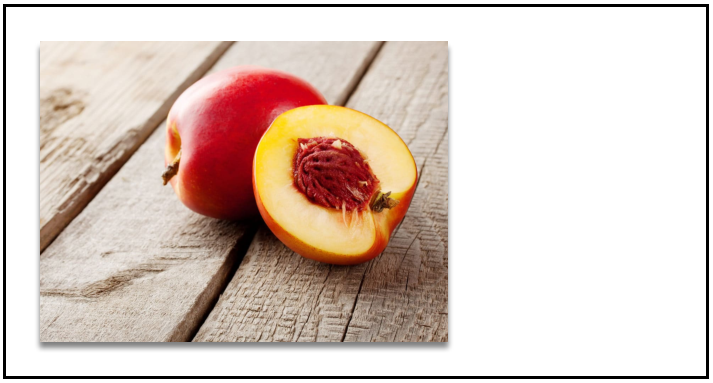
\includegraphics[scale=0.8]{./figures-pdf/peach_1}<1>
	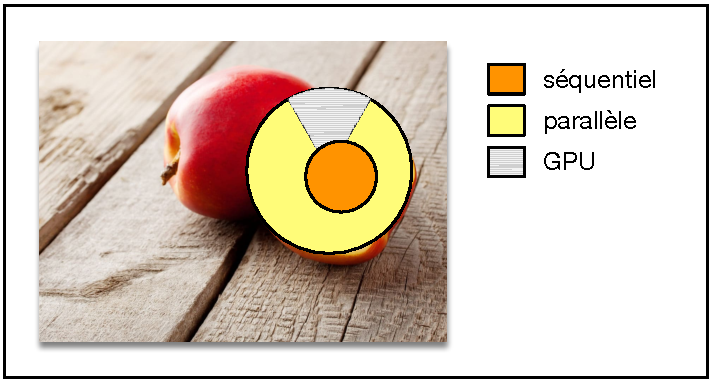
\includegraphics[scale=0.8]{./figures-pdf/peach_2}<2>
	
	{\tiny Exemple tiré de Programming Massively Parallel Processors}
	\end{center}
\end{frame}
%%%%%%%%%%%%%%%%%%%%%%%%%%


%%%%%%%%%%%%%%%%%%%%%%%%%%%
\subsection{Domaines d'utilisation et languages}
\begin{frame}{Plan}
\tableofcontents[sections={1-4}, currentsubsection]
\end{frame}
%%%%%%%%%%%%%%%%%%%%%%%%%%%


%%%%%%%%%%%%%%%%%%%%%%%%%%
\begin{frame}[plain]
\frametitle{Domaines d'application du calcul parallèle}
	\begin{center}
	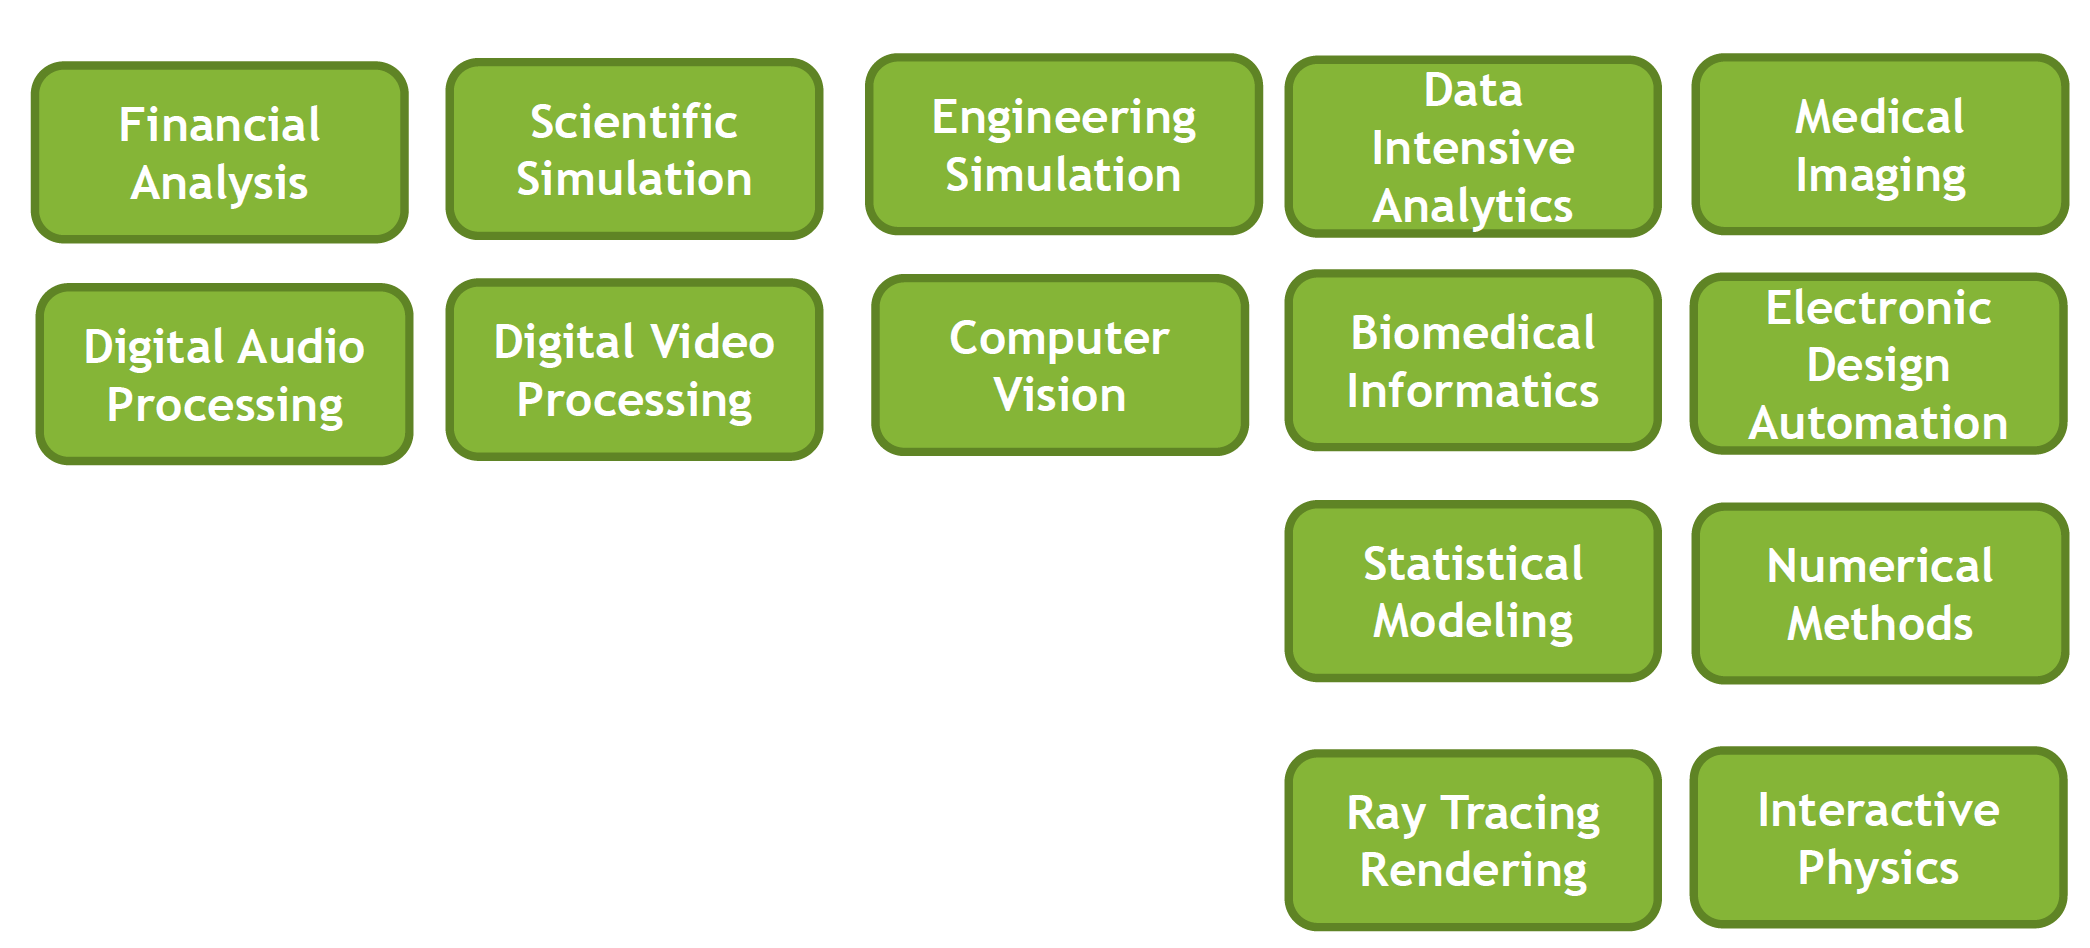
\includegraphics[scale=0.3]{./figures-pdf/domaines}
	
	{\tiny [Lecture 1.2 Heterogenous computing, GPU Teaching Kit Nvidia]}
	\end{center}

\end{frame}
%%%%%%%%%%%%%%%%%%%%%%%%%%
\begin{frame}[plain]
\frametitle{La programmation de GPU}
\centering
Trois façon de développer des applications sur GPU

\begin{columns}[t]
  \begin{column}{0.32\textwidth}
  \uncover<1,2,5>{
    \begin{block}{Utilisation de bibliothèques}
        \uncover<2,5>{
	\begin{itemize}
		\item Facile à utiliser
		\item Performant
		\item Qualité
	\end{itemize}
	}
\end{block}   
}
  \end{column}
  

  \begin{column}{0.32\textwidth}
    \uncover<1,3,5>{
    \begin{block}{Directives de compilation}
        \uncover<3,5>{
    	\begin{itemize}
		\item  Facile à utiliser
		\item Code portable
		\item Perf. incertaines
		}
	\end{itemize}
    \end{block}  
    }
  \end{column}

  
    \begin{column}{0.32\textwidth}
      \uncover<1,4,5>{
    \begin{block}{Langage de programmation}
        \uncover<4,5>{
    	\begin{itemize}
		\item  Performant
		\item Flexible
		\item Verbeux
	\end{itemize}
	}
    \end{block}  
    }
  \end{column}
 \end{columns}
 
 	\begin{center}
	
\includegraphics[scale=0.5]{./figures-pdf/empty}<1,5>
	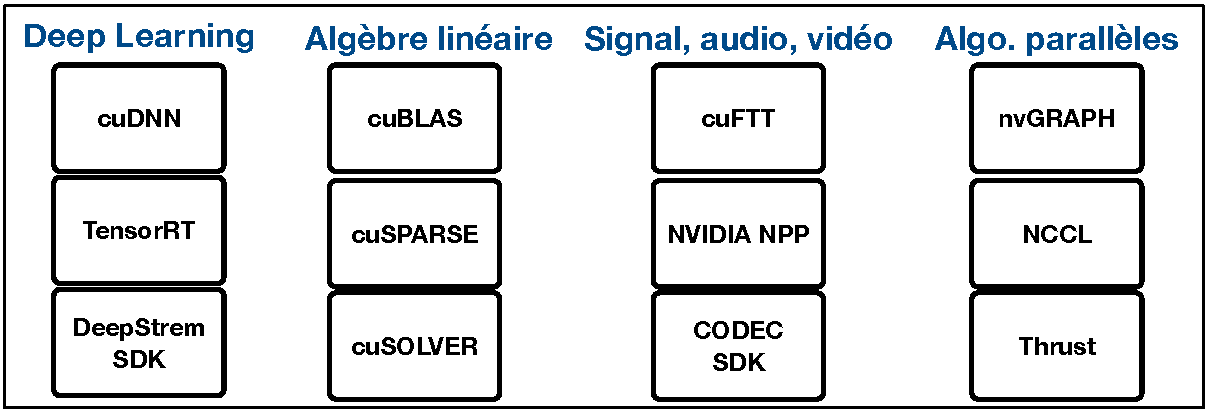
\includegraphics[scale=0.5]{./figures-pdf/lib}<2>
	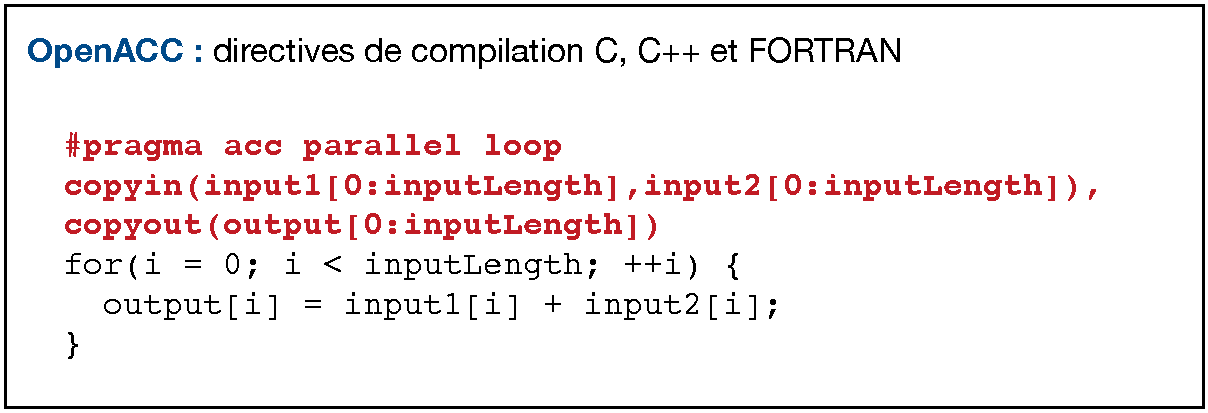
\includegraphics[scale=0.5]{./figures-pdf/directives}<3>
	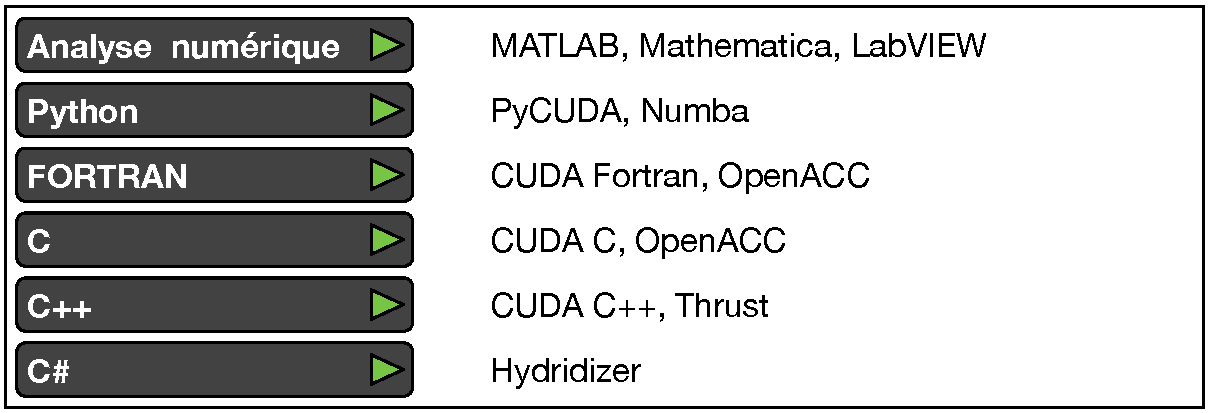
\includegraphics[scale=0.5]{./figures-pdf/langages}<4>
	\end{center}
\end{frame}
%%%%%%%%%%%%%%%%%%%%%%%%%%


%%%%%%%%%%%%%%%%%%%%%%%%%%%
\subsection{Le langage CUDA-C}
\begin{frame}{Plan}
\tableofcontents[sections={1-4}, currentsubsection]
\end{frame}
%%%%%%%%%%%%%%%%%%%%%%%%%%%

%%%%%%%%%%%%%%%%%%%%%%%%%%%
\begin{frame}[plain]
\frametitle{CUDA-C}
\begin{itemize}
	\item NVIDIA fournit un compilateur CUDA-C : nvcc
	\item nvcc compile le code pour le GPU puis le transmet au compilateur hôte (par exemple {\tt g++})
	\item Peut être utilisé pour compiler et éditer les liens des applications réservées à l'hôte (i.e. CPU)
	\item Outils de débug : Nsight, CUDA-GDB, CUDA MEMCHECK
	\item Outils de profilage de performance : Nsight, NVVP, NVPROF, NVTX
\end{itemize}
\end{frame}

%%%%%%%%%%%%%%%%%%%%%%%%%%
\begin{frame}[plain]
\frametitle{Structure d'un programme C en CUDA}
%
\begin{block}{{\it host} et {\it device}}
Un programme CUDA fait coexister du code pour deux éléments d'exécution un {\bf host} (CPU) et un ou plusieurs  {\bf devices} (GPUs).

Par défaut le code C est écrit pour le \host, mais des mots-clefs dédiés vont permettre de spécifier qu'une portion de code est dédiée aux {\it devices}.
\end{block}

\begin{block}{Chaîne de compiltation}
\center	
\includegraphics[scale=0.5]{./figures-pdf/compilation}
\end{block}

\end{frame}


%%%%%%%%%%%%%%%%%%%%%%%%%%
\begin{frame}[plain]
\frametitle{Exécution d'un programme C en CUDA}
%

\begin{block}{Principe d'exécution : fonction et kernel}
\center	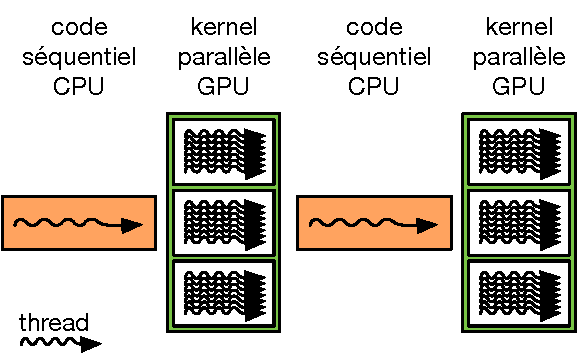
\includegraphics[scale=0.7]{./figures-pdf/execution}
\end{block}
\end{frame}

%%%%%%%%%%%%%%%%%%%%%%%%%%%
\subsection{Architecture matérielle pour la pratique}
\begin{frame}{Plan}
\tableofcontents[sections={1-4}, currentsubsection]
\end{frame}
%%%%%%%%%%%%%%%%%%%%%%%%%%%

%%%%%%%%%%%%%%%%%%%%%%%%%%
\begin{frame}[plain]
\frametitle{Architecture matérielle utilisée : Jetson Nano}
%
\begin{columns}[t]
  \begin{column}{0.45\textwidth}

    \begin{center}
	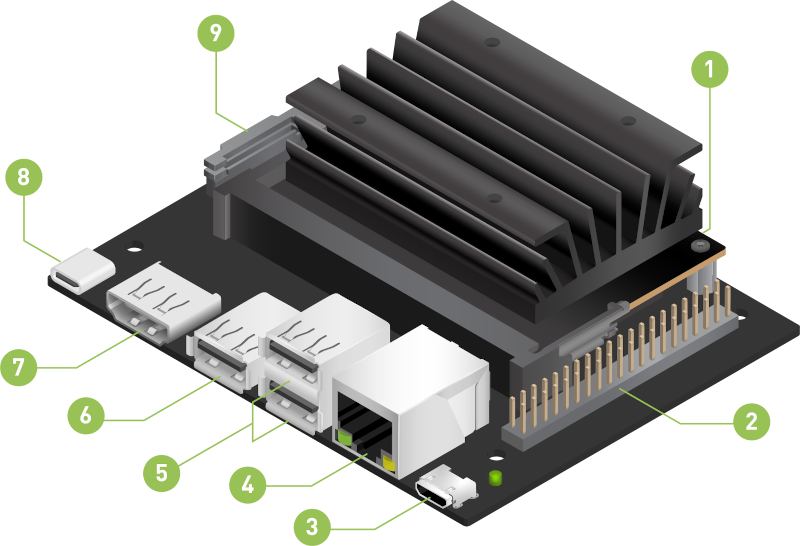
\includegraphics[scale=0.3]{./figures-pdf/jetson}
    \end{center}	
  \end{column}
  
  \begin{column}{0.55\textwidth}
    \begin{block}{Architecture}
    \begin{center}
	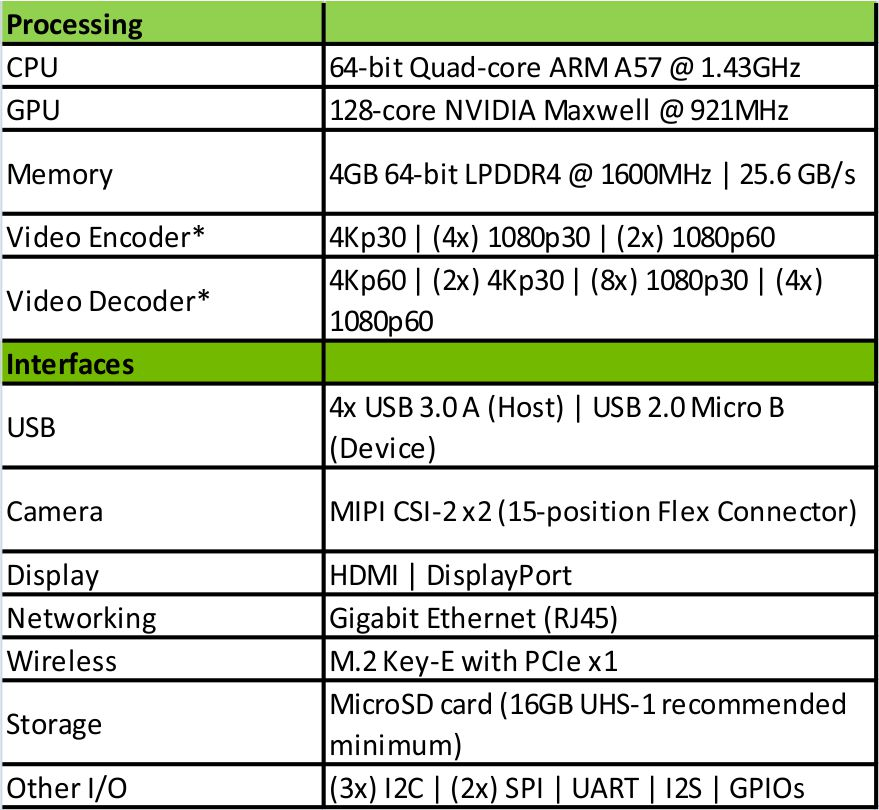
\includegraphics[scale=0.8]{./figures-pdf/jetson-nano_spesification_epsindo-1}
    \end{center}	
	  \end{block}   
  \end{column}
 \end{columns}  
 
\end{frame}
%%%%%%%%%%%%%%%%%%%%%%%%%%
\begin{frame}[plain]
\frametitle{Architecture matérielle utilisée : Jetson Nano}
%
    \begin{center}
	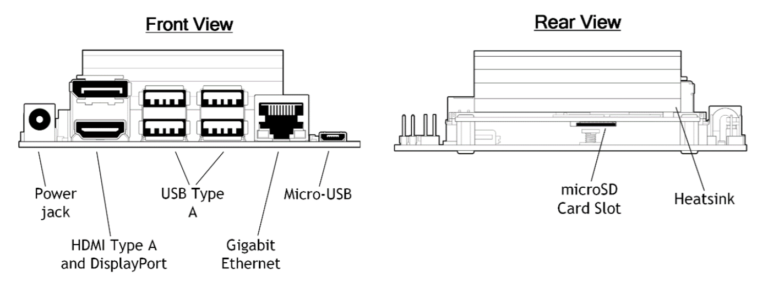
\includegraphics[width=\textwidth]{./figures-pdf/front}<1>
%	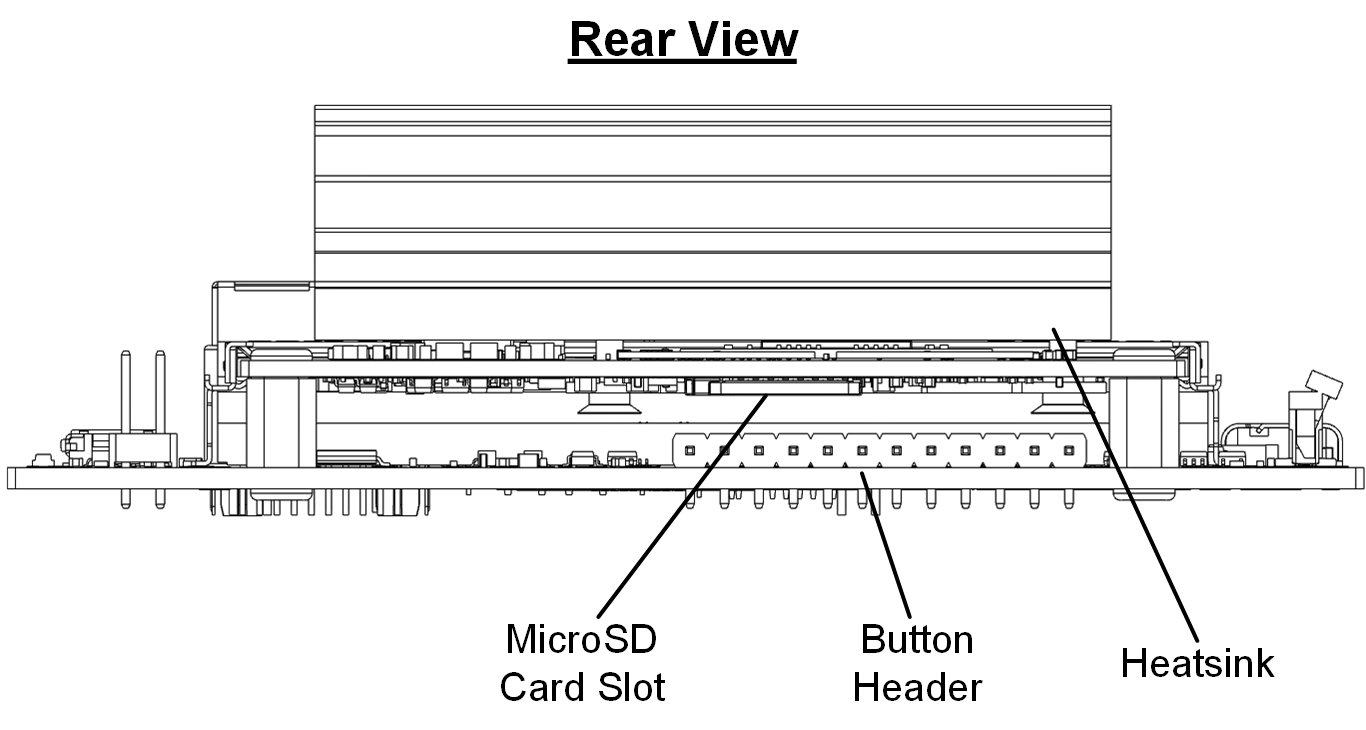
\includegraphics[width=\textwidth]{./figures-pdf/rear}<2>
	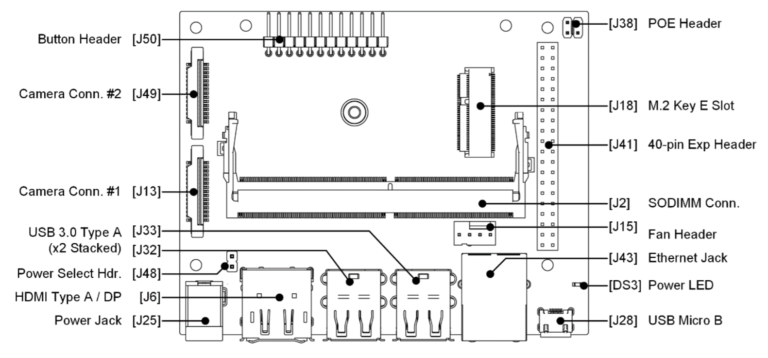
\includegraphics[width=\textwidth]{./figures-pdf/top}<2>
    \end{center}	
 
\end{frame}

%%%%%%%%%%%%%%%%%%%%%%%%%%
\begin{frame}[plain]
\frametitle{Un peu de pratique avec le TD1}

\begin{block}{Objectifs}
\begin{itemize}
	\item Installer les outils (si ce n'est pas déjà fait)
	\item Compiler avec {\tt nvcc} et exécuter un code sur un GPU
	\item Récupérer et afficher les informations du {\it device}
\end{itemize}
\end{block}
\end{frame}
%%%%%%%%%%%%%%%%%%%%%%%%%%

\section{Allocation des données et exécution d'un kernel}
\section{Kernel à plusieurs dimensions}


\end{document}